\RequirePackage[OT1]{fontenc} 
\documentclass[journal]{IEEEtran}

% *** CITATION PACKAGES ***
\usepackage[style=ieee]{biblatex} 
\bibliography{example_bib.bib}    %your file created using JabRef

% *** MATH PACKAGES ***
\usepackage{amsmath}

% Table Packages
\usepackage{booktabs}
\usepackage{tabularx}

% *** PDF, URL AND HYPERLINK PACKAGES ***
\usepackage{url}
% correct bad hyphenation here
\hyphenation{op-tical net-works semi-conduc-tor}
\usepackage{graphicx}  %needed to include png, eps figures
\graphicspath{{./images/}}
\usepackage{float}  % used to fix location of images i.e.\begin{figure}[H]

\begin{document}

% paper title
\newcommand{\LabNumber}{\#7}
\newcommand{\LabTitle}{RF Filters}

\title{RF Lab Module \LabNumber\ --- \LabTitle}
%\\ \small{Title of the session (you can be creative highlighting your findings)}}

% author names 
\author{Stephen Campbell
    % Student 2 First Name Last Name 
}% <-this % stops a space

% The report headers
\markboth{EE/CE 4202 Electrical and Computer Engineering Laboratory in Circuits. Lab \LabNumber, \today}%do not delete next lines
{Shell \MakeLowercase{\textit{et al.}}: Bare Demo of IEEEtran.cls for IEEE Journals}

% make the title area
\maketitle

% As a general rule, do not put math, special symbols or citations
% in the abstract or keywords.
\begin{abstract}
    RF filters are of immense importantance in today's RF dependent world. Nearly
    every consumer electronic device utilized RF filters to communicate and connect
    with the internet. In this lab, several RF filters were designed, characterized,
    and analyzed. Specifically,  a 0.5dB equal ripple low pass filter was implemented
    using the stepped impedance method.
\end{abstract}

\section{Introduction}

\IEEEPARstart{I}{mplementing} Implementing a stepped impedance low pass filter
requires a desired filter order and cutoff frequency. In this lab, we designed 2
5th order low pass filters with a cutoff frequency of 600Mhz and 1.2GHz. The
e design made use of the low-pass filter prototype charts. This made choosing
component values as simple as calculating an equation. These filters where
chartered by measuring the S parameters across frequency.

\section{Procedure}
\begin{enumerate}
    \item Compute Design Parameters
          \begin{enumerate}
              \item Determine \(Z_{\text{low}}\), \(Z_{\text{high}}\)
              \item Use prototype elements to determine desired inductor and capacitor values
              \item Determine the TX line length required to realize the passives
          \end{enumerate}
    \item Manufacture Filter
          \begin{enumerate}
              \item Cut copper tape strips to width determined by \(Z_{\text{low}}\),
                    \(Z_{\text{high}}\)  and length determined by length needed by passives
              \item Adhere the copper strips to blank side of copper-plated FR4 board to
                    realize the stepped impedance configuration
              \item Solder SMA connectors to either end adding 50Ohm microstrip line to extend where necessary
          \end{enumerate}
    \item Characterize Filter
          \begin{enumerate}
              \item Calibrate VNA with 201 points from 50k-3GHz
          \end{enumerate}
\end{enumerate}

\section{Analysis}
\textbf{Record the observations and conclusions from the lab.}
The 600Mhz filter behaved as expected with a cutoff frequency around 600Mhz;
however, the effects of the transmission line properties of the stepped
impedance were exposed.  After \~1.4GHz the filter started to pass the signal
once again with ripples following after the resurgence. The milled stepped
impedance filter proved to have an exceptionally flat pass bad; however, due to
the limited calibration frequencies the filter gave poor results outside of
3GHz. The lack of calibration outside of 3GHz is cited for the apparent chaotic
transfer charactistics for the milled stepped impedance filter.

\begin{figure}
    \centering
    \includegraphics[width=0.3\textwidth]{600MHz_rl.png}
    \caption{Measured S Parameters of DIY \(f_c=600\)MHz Stepped Impedance Low Pass Filter}
\end{figure}

\begin{figure}
    \centering
    \includegraphics[width=0.3\textwidth]{AWR_600.png}
    \caption{Theoretical S Parameters of 600Mhz filter compared with Measured S Parameters}
\end{figure}

\begin{figure}
    \centering
    \includegraphics[width=0.3\textwidth]{unkown_rl.png}
    \caption{Measured S Parameters of Unknown Cutoff frequency Milled Stepped Impedance Low Pass Filter}
\end{figure}

\begin{table}[hp]
    \centering
    \begin{tabularx}{0.5\textwidth}{XXXXX}
        \toprule
        Parameter                               & TX line (0.6   GHz) & TX Line (1.2   GHz) & Measured 0.6   GHz & Milled T line \\ \midrule
        Ripple                                  & 0.885dB             & 0.8782 dB           & 0.96dB             & N/A           \\ \midrule
        Cutoff   frequency (3dB)                & 574MHz              & 1135MHz             & 557.7MHz           & 2273MHz       \\ \midrule
        Rejection at   1.2 GHz                  & 12.72dB             & 1.6dB               & 15.14dB            & In Passband   \\ \midrule
        Min. Return   loss (dB) across the band & -58.42dB            & -64.48              & -58.42dB           & -61.1dB       \\ \bottomrule
    \end{tabularx}

    \vspace{1em}
    \caption{Recorded Values of Simulated and Measured Filters}
    \label{tab:records}
\end{table}



\textbf{How do your measured values compare with the simulated responses (\% error). What might be causing the error?}

\begin{table}[hp]
    \centering
    \begin{tabular}{lll}
        \toprule
        \multicolumn{3}{c}{600 MHz Filter} \\ \midrule
        Measured  & Actual   & \% Error    \\ \midrule
        0.96 dB   & 0.885 dB & 8.474576    \\ \midrule
        557.7 MHz & 574MHz   & 2.839721    \\ \midrule
        15.14 dB  & 12.72 dB & 19.02516    \\ \midrule
        58.42 dB  & 58.42 dB & 0           \\ \bottomrule
    \end{tabular}

    \vspace{1em}
    \caption{Percent Error of Measured vs. Simulated Values for the 600MHz filter}
    \label{tab:600_error}
\end{table}
There are several factors that could contribute to the error between the
simulated and measured values. For example, the manufacturing accuracy,
differences between the different board parameters such as \(\tan(\delta) \) or
board height, and systematic measurement error.

\textbf{How long did it take you to complete the lab?}

1 hour 15 minutes

\section{Discussion and Summary}

Overall, this lab exposed the tradeoffs leveraged when designing RF filters
including the properties of TX lines, accuracy of manufacturing processes, and
difference between passives realized by lumped vs.\ distributed methods.
Experience as gained using the stepped impedance method to realize a 0.5dB
Chebyshev 5th low pass filter.

\appendices
% \section{Pre-Lab}

\begin{table}[]
    \centering
    \begin{tabular}{lll}
        \toprule
        Z0 (Ohm) & Width (mil) & Width (cm) \\ \midrule
        20       & 474.84      & 1.20609    \\ \midrule
        50       & 132.87      & 0.33749    \\ \midrule
        55       & 113.13      & 0.28735    \\ \bottomrule
    \end{tabular}

    \vspace{1em}
    \caption{Width of microstrip transmission lines}
    \label{tab:tx_dims}
\end{table}

\begin{table}[]
    \centering
    \begin{tabular}{ll}
        \toprule
        \(g_1\) & 1.7058 \\ \midrule
        \(g_2\) & 1.2296 \\ \midrule
        \(g_3\) & 2.5408 \\ \midrule
        \(g_4\) & 1.2296 \\ \midrule
        \(g_5\) & 1.7058 \\ \midrule
        \(g_6\) & 1      \\ \bottomrule
    \end{tabular}

    \vspace{1em}
    \caption{Prototype Parameters of 0.5dB Equal Ripple Low pass Filter}
    \label{tab:prototype_params}
\end{table}

\begin{table}[]
    \centering
    \begin{tabularx}{0.5\textwidth}{XXXX}
        \toprule
        Component & Electrical   Length in Radians & Length (cm) of   MS TX Line 600MHz & Length (cm) of   MS TX Line 1.2GHz \\ \midrule
        C1        & 0.68232                        & 2.85605                            & 1.42423                            \\ \midrule
        L1        & 1.2296                         & 4.9972                             & 2.48582                            \\ \midrule
        C2        & 1.01632                        & 4.2541                             & 2.1214                             \\ \midrule
        L2        & 1.2296                         & 4.9972                             & 2.48582                            \\ \midrule
        C3        & 0.68232                        & 2.85605                            & 1.42423                            \\ \bottomrule
    \end{tabularx}

    \vspace{1em}
    \caption{Filter Components and Corresponding TX line lengths}
    \label{tab:tx_dims_2}
\end{table}

\section{Extra Photos}

\begin{figure}[hp]
    \centering
    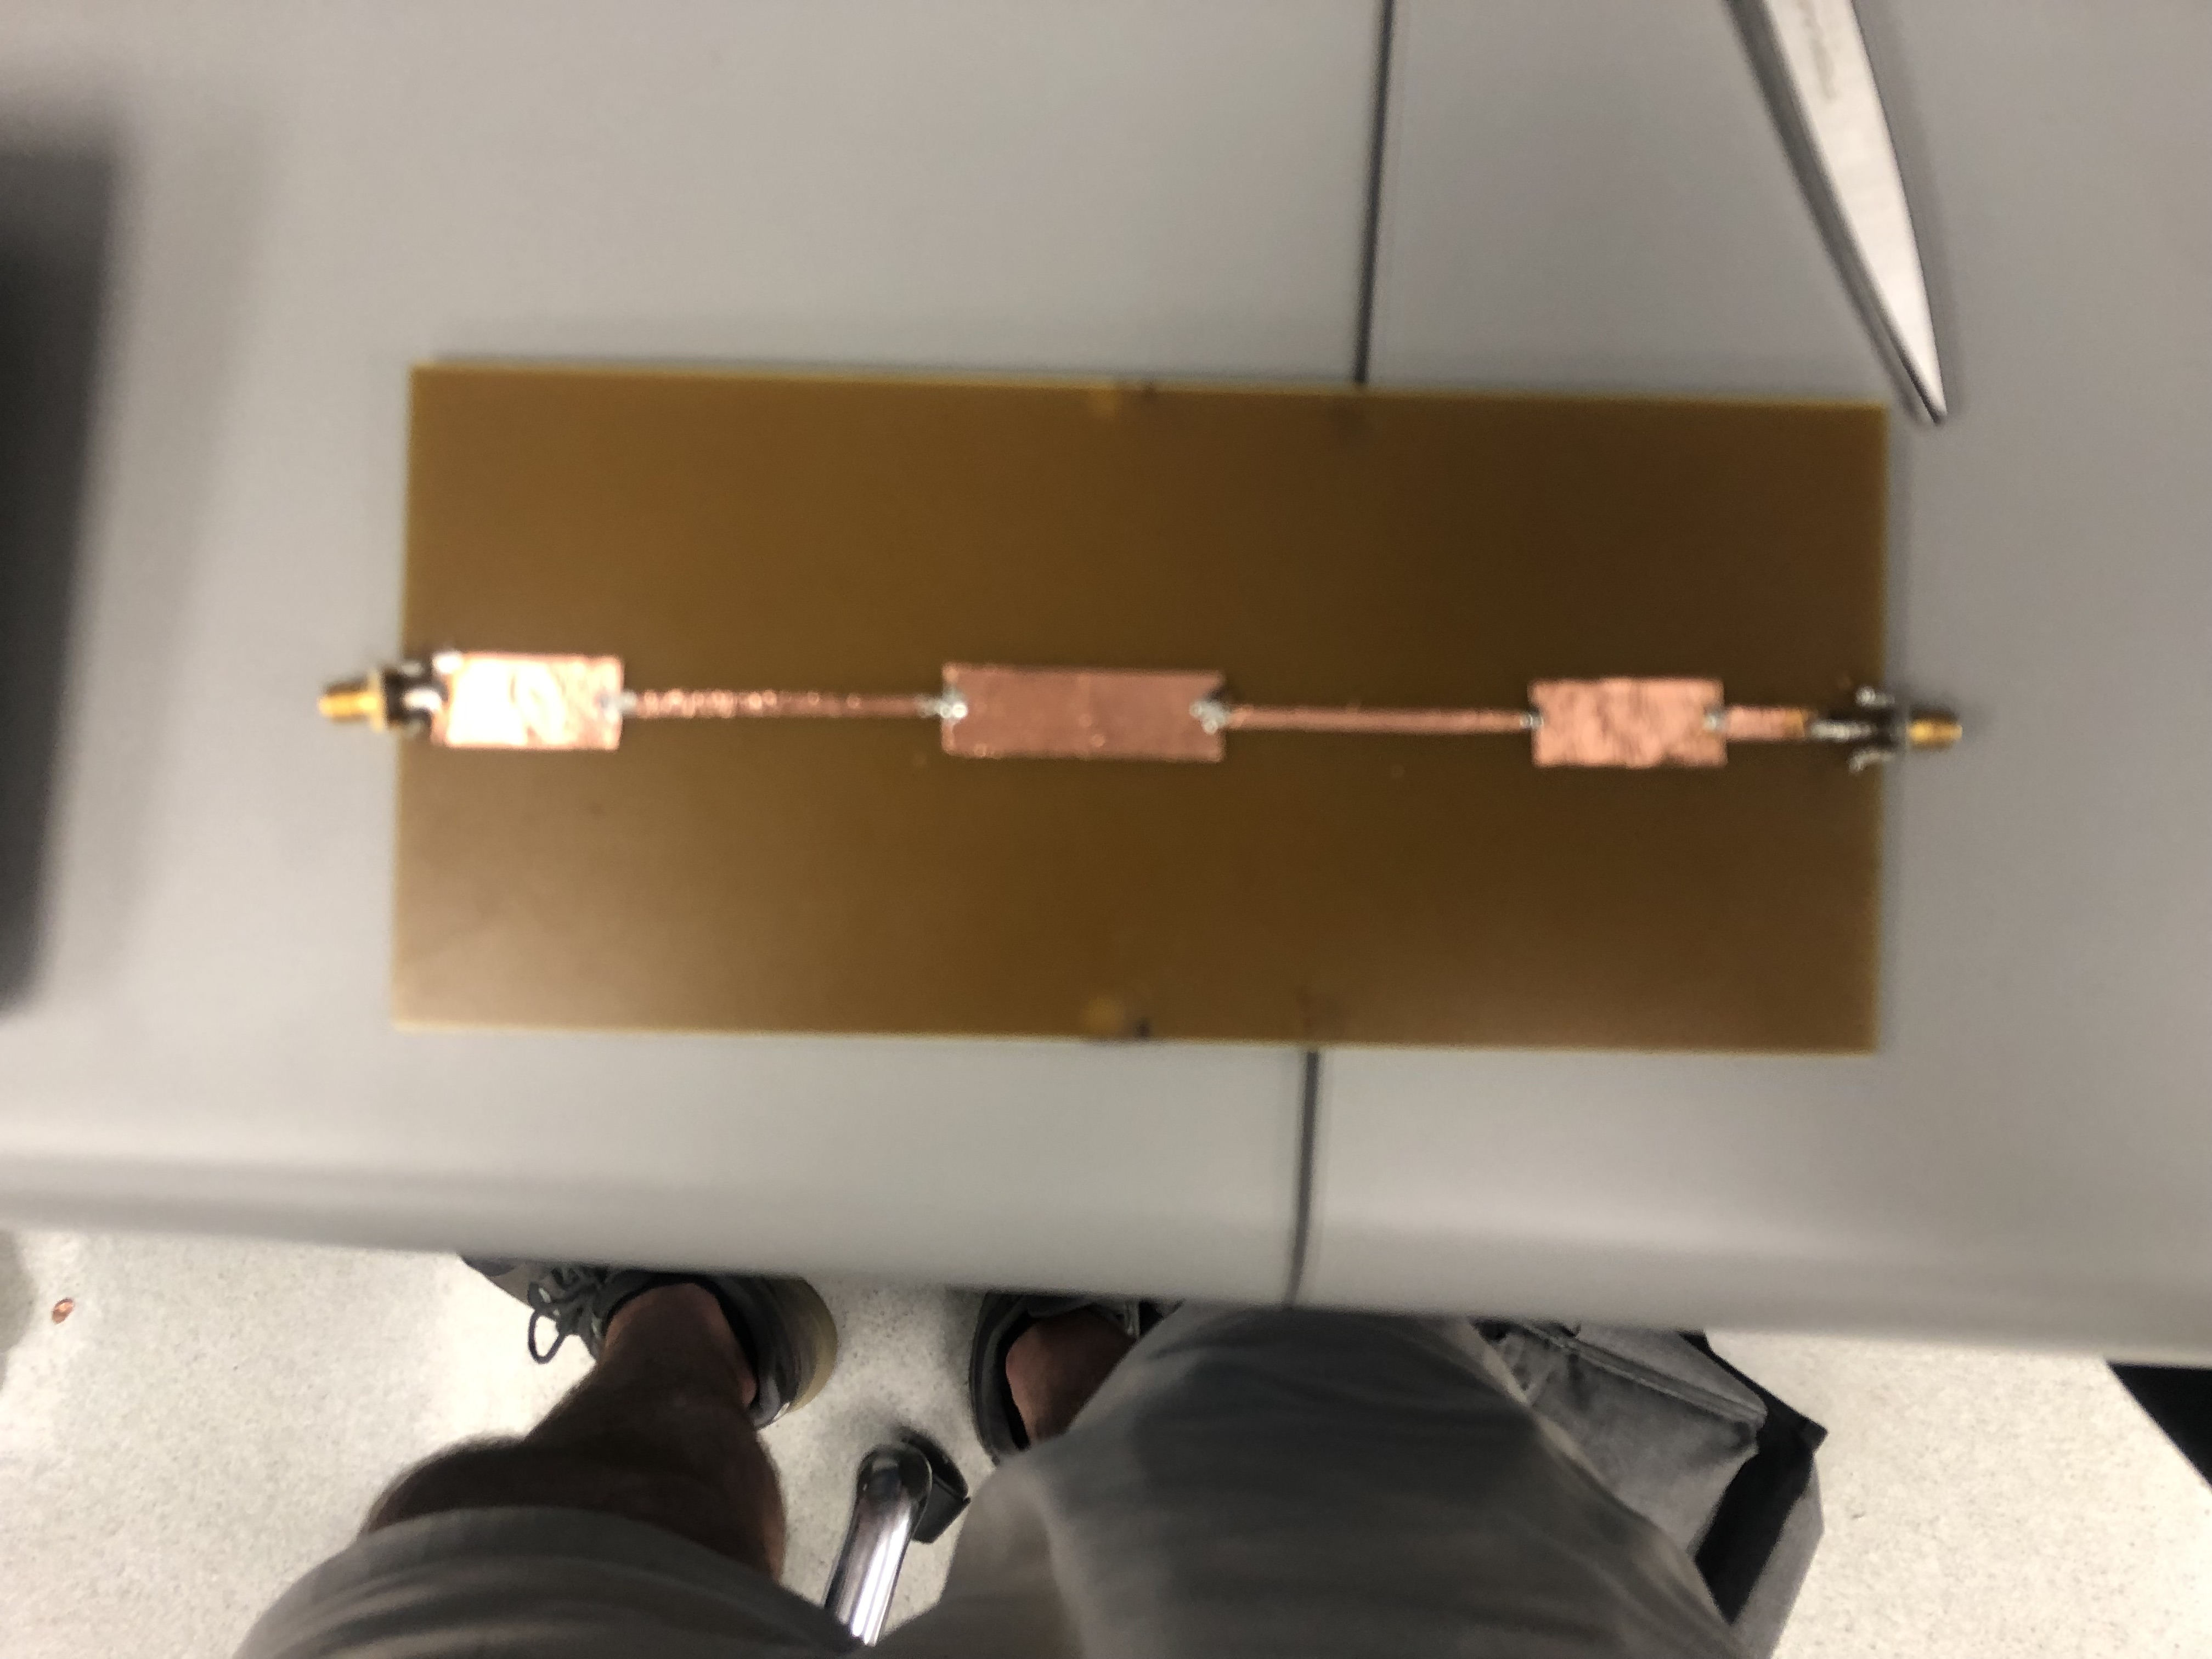
\includegraphics[width=0.3\textwidth]{diy_filter.png}
    \caption{Copper Tape 600MHz Filter}
\end{figure}

\begin{figure}[hp]
    \centering
    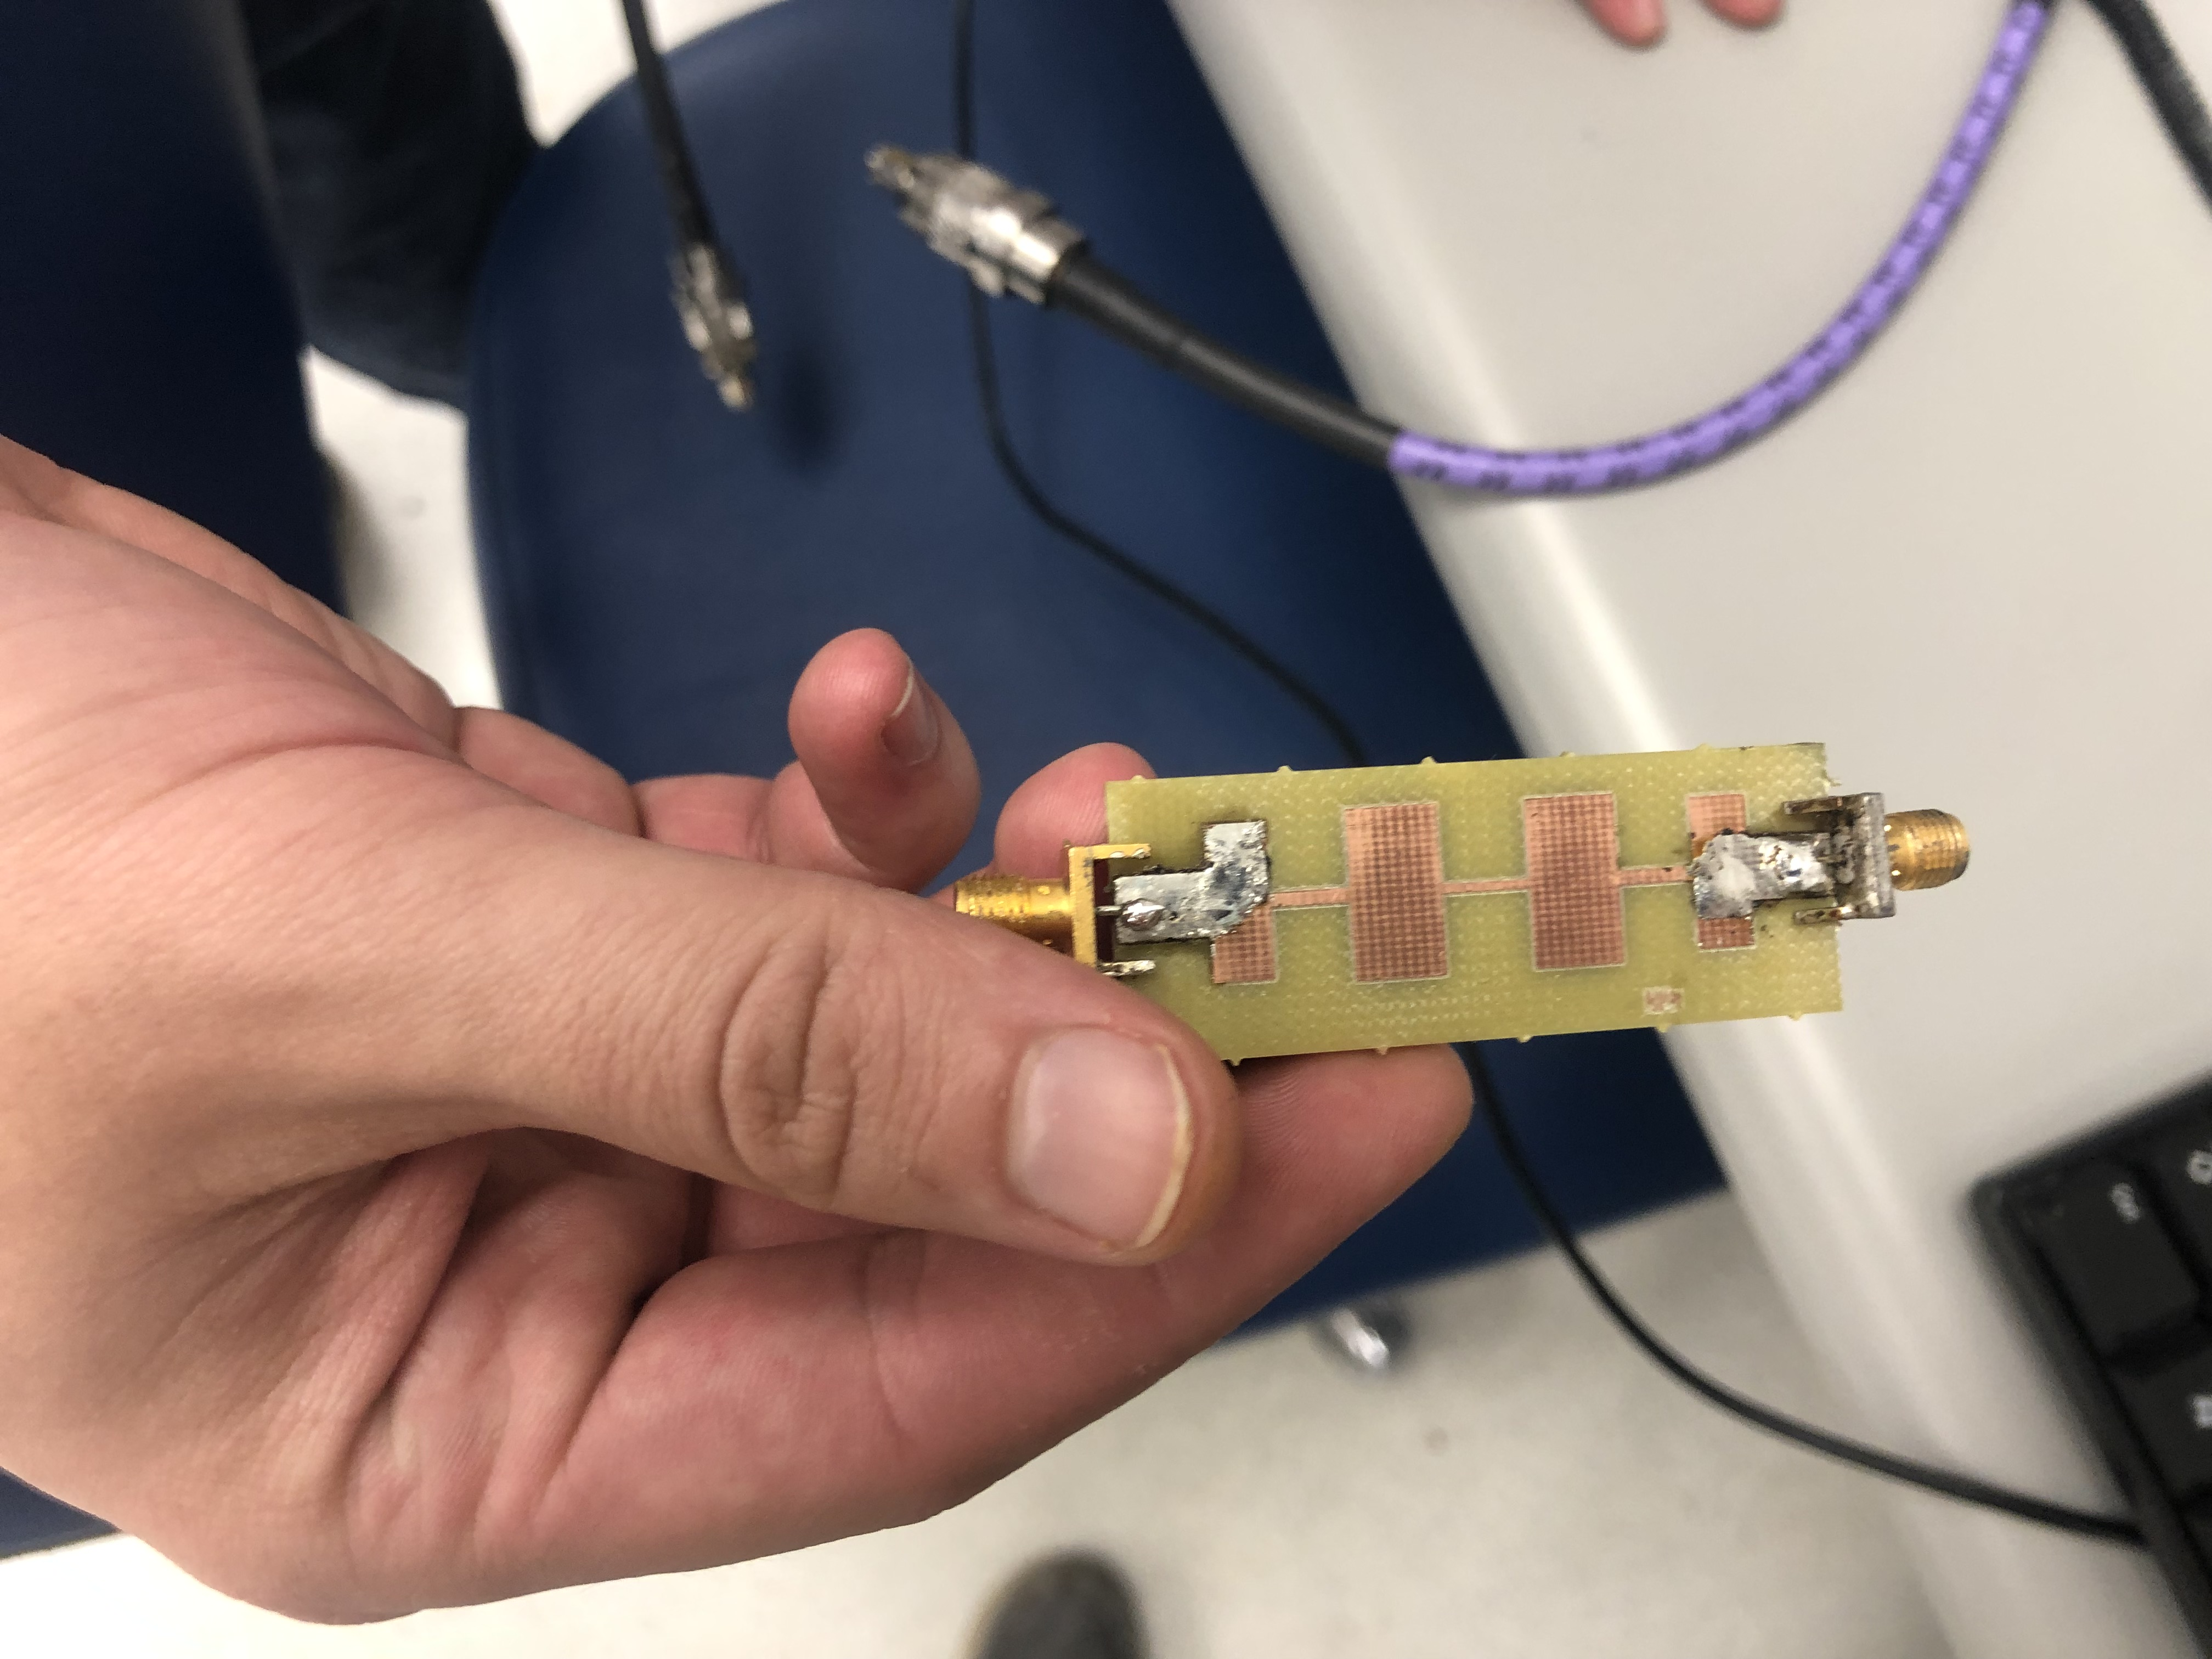
\includegraphics[width=0.3\textwidth]{milled_filter.png}
    \caption{Milled Filter}
\end{figure}

\end{document}